\documentclass{article}
\usepackage[utf8]{inputenc}
\usepackage{graphicx}
\usepackage{subcaption}
\usepackage{amsmath}

\title{Image and Video Processing Lab 3}
\author{Philine Witzig}
\date{November 2020}

\begin{document}

\maketitle
General notes: when running the matlab script, you will be asked to enter the number of the task you want to test. Enter the numbers $1$ to $4$ in order to test the respective edge detectors. In Section \ref{sec:discussion}, you can find an evaluation of the above methods.

\section{Template Method}
For the template method, the function \textsf{edge\_detect\_template(I, g1, g2, norm, thresh)} was implemented. It receives the following parameters: an input image \textsf{I}, the template for vertical edges \textsf{g1} and the one for horizontal edges \textsf{g2}, a String \textsf{norm} (either ``L1" or ``L2") indicating the norm which will be used for magnitude approximation and a threshold value \textsf{thresh} between $0$ and $25$ for separating edge from non-edge pixels. The function applies the vertical and the horizontal filter using matlab's 2D convolution function as \textsf{conv2(I, filter, 'same')}, which convolves the input image \textsf{I} with \textsf{filter} while keeping the dimensions the same. The magnitude is then computed from the two filtered images depending on the passed norm. Edge pixels are then filtered using matlab's function \textsf{imbinarize(I, thresh)}, where \textsf{I} is the magnitude now.

\paragraph{Discussion} Figure \ref{fig:temp_sobel_lena} show the results on \textsf{lena.png} for different norms using the Sobel filter and a threshold of $25$, which was determined empirically such that the result would preserve the contours of Lena. What we can observe is that there is more noise in the L1 approximation compared to when L2 is used. At the same time, L2 also removes some edges in the background. Figure \ref{fig:temp_filters_lena} additionally compares the results when the Prewitt and Roberts filter were used (L2 approx., \textsf{thresh} = $25$). While Prewitt achieves a result comparable to Sobel, Roberts removed many edges in the background. Based on these findings, Sobel with L2 approximation was also applied to \textsf{rice.png} and \textsf{road.png} (cf. Figure \ref{fig:temp_rice_road}). For \textsf{rice.png}, very precise edge detection (corresponding to contour here) is possible since there is no noise in the background. 
\begin{figure}
        \centering
        \begin{subfigure}[b]{0.49\textwidth}
            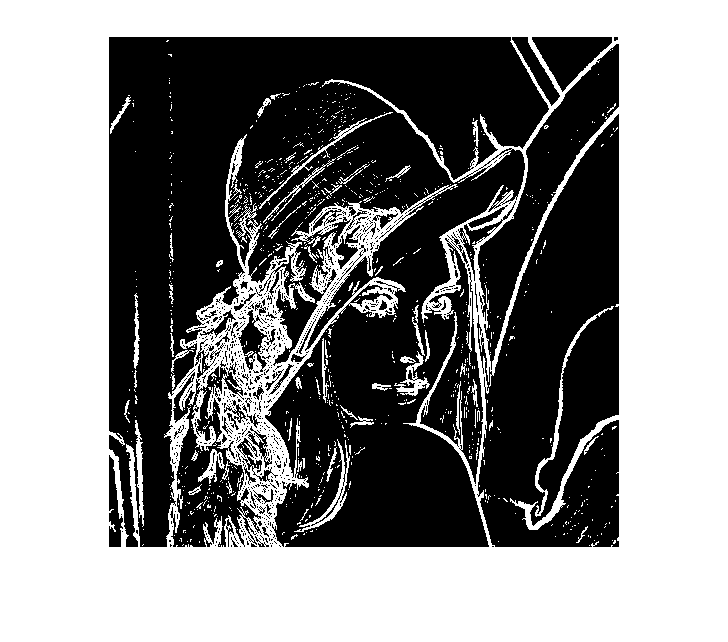
\includegraphics[width=\textwidth]{Images/lena_sobel_l1.png}
            \subcaption{L1 approximation}
        \end{subfigure}
        \begin{subfigure}[b]{0.49\textwidth}
            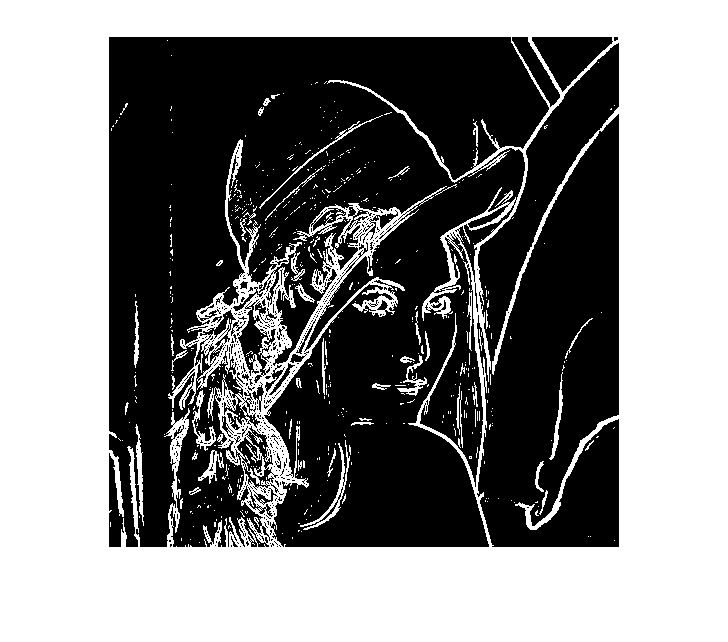
\includegraphics[width=\textwidth]{Images/lena_sobel_l2.png}
            \subcaption{L2 approximation}
        \end{subfigure}
        \caption{Results of template based method using Sobel on \textsf{lena.png} with different norms for magnitude approximation.}
        \label{fig:temp_sobel_lena}
\end{figure}

\begin{figure}
        \centering
        \begin{subfigure}[b]{0.49\textwidth}
            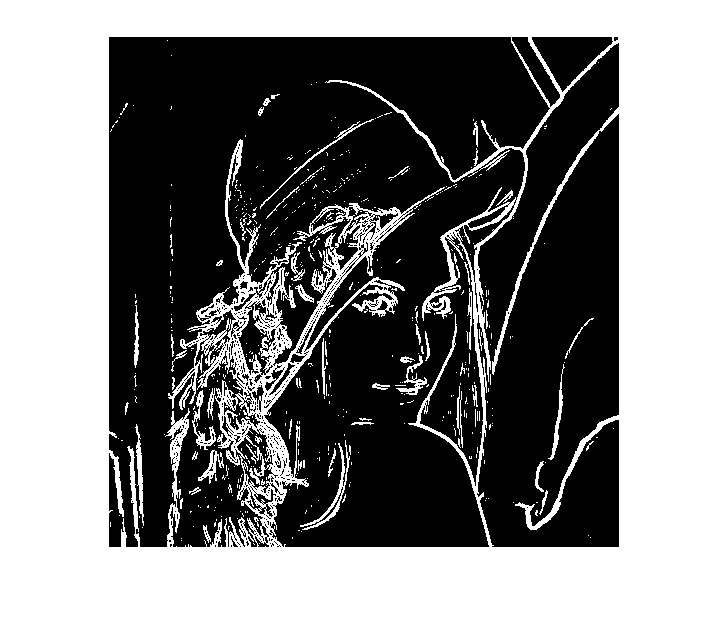
\includegraphics[width=\textwidth]{Images/lena_prewitt_l2.png}
            \subcaption{Prewitt}
        \end{subfigure}
        \begin{subfigure}[b]{0.49\textwidth}
            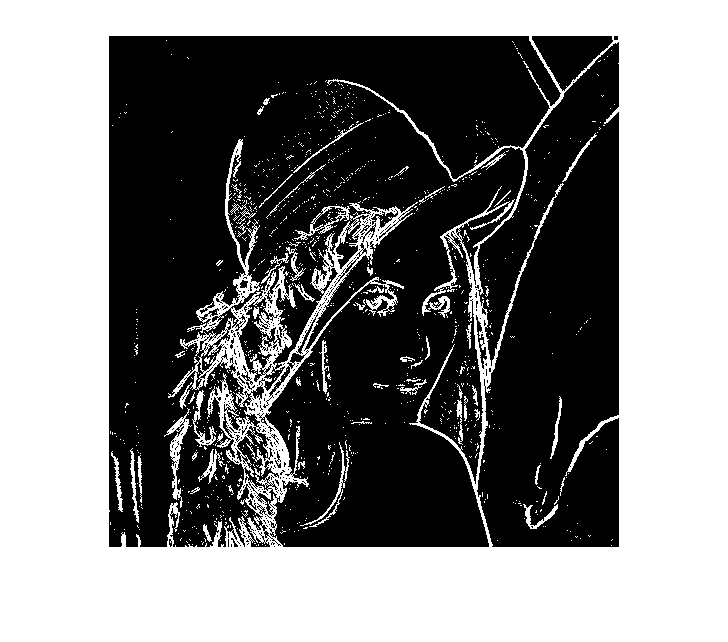
\includegraphics[width=\textwidth]{Images/lena_roberts_l2.png}
            \subcaption{Roberts}
        \end{subfigure}
        \caption{Results of template based method using Prewitt and Roberts on \textsf{lena.png} with L2.}
        \label{fig:temp_filters_lena}
\end{figure}

\begin{figure}
        \centering
        \begin{subfigure}[b]{0.45\textwidth}
            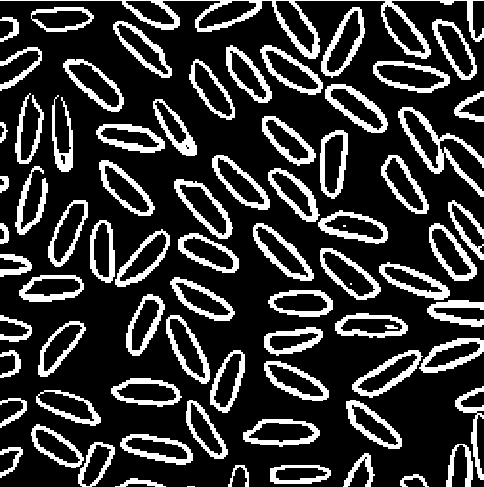
\includegraphics[width=\textwidth]{Images/rice_sobel_l2.png}
            \subcaption{Sobel, L2, 32}
        \end{subfigure}
        \hfill
        \begin{subfigure}[b]{0.45\textwidth}
            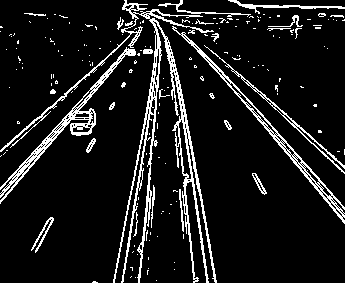
\includegraphics[width=\textwidth]{Images/road_sobel_l2.png}
            \subcaption{Sobel, L2, 30}
        \end{subfigure}
        \caption{Results of template based method with Sobel and L2 on \textsf{rice.png} and \textsf{road.png} with different thresholds.}
        \label{fig:temp_rice_road}
\end{figure}


\section{Compass Operator}
Edge detection using the compass operator works by looking at the gradient in multiple directions. This is achieved by having one reference filter which is rotated by a factor of $45 ^ \circ$. In this submission, edge detection using the compass operator is implemented in \textsf{edge\_detect\_compass(I, mask, thresh)}, where \textsf{I} is the input image, \textsf{mask} is the reference filter which will be rotated, \textsf{thresh} is the threshold value for separating edge from non-edge pixels. The rotation is achieved using matlab's \textsf{ imrotate(mask, 45 $\cdot$ c, 'crop')} function where \textsf{c} $\in \{ 1 \dots 7 \}$ and the parameter \textsf{'crop'} ensures that we still obtain a square filter (and not a diamond) when \textsf{c} is uneven. The filter is applied as in the previous task. We then select the elementwise max. absolute pixel value for the different filtered images using matlab's \textsf{max(\dots)} function. Last but not least, edge pixels are separated from non-edge pixeels using \textsf{imbinarize(I, thresh)}, where \textsf{I} is the magnitude now.

\paragraph{Discussion}
Figure \ref{fig:compass} visualizes the result when the compass method was used, keeping the thresholds as in the previous exercise. Although the compass method is capable of capturing more edge directions, i.e. $8$, we cannot observe any significant visual differences to the outputs of the Sobel filter with L2 approximation. 
\begin{figure}
        \centering
        \begin{subfigure}[b]{0.32\textwidth}
            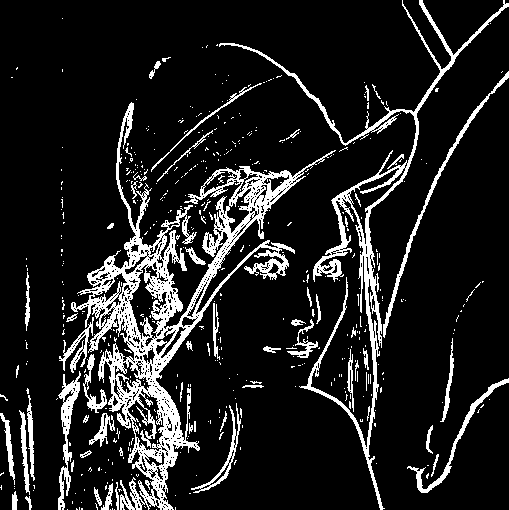
\includegraphics[width=\textwidth]{Images/lena_compass.png}
            \subcaption{thresh=25}
        \end{subfigure}
        \hfill
        \begin{subfigure}[b]{0.32\textwidth}
            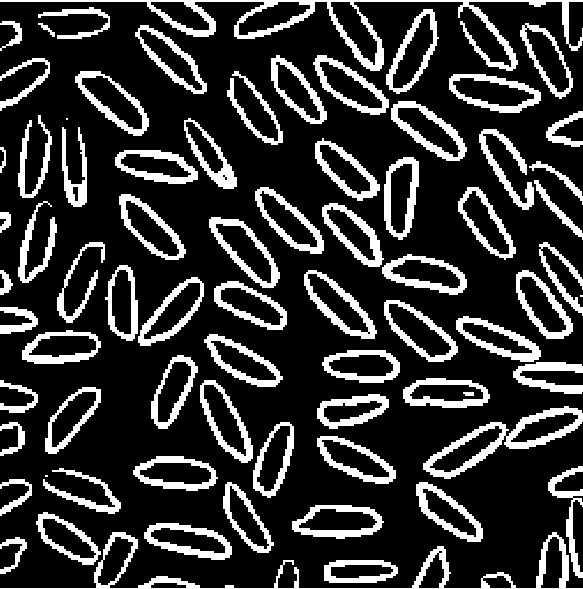
\includegraphics[width=\textwidth]{Images/rice_compass.png}
            \subcaption{thresh=32}
        \end{subfigure}
        \hfill
        \begin{subfigure}[b]{0.32\textwidth}
            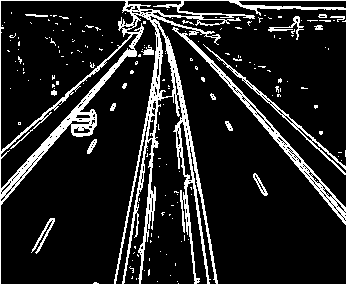
\includegraphics[width=\textwidth]{Images/road_compass.png}
            \subcaption{thresh=30}
        \end{subfigure}
        \caption{Results of compass method on \textsf{lena.png}, \textsf{rice.png} and \textsf{road.png} with different thresholds.}
        \label{fig:compass}
\end{figure}

\section{Laplace Operator}
For the LoG edge detection, the filter is created using \textsf{fspecial('log', hsize, $\sigma$)}. The filter size is determined by \textsf{hsize} = $2 \cdot \lceil 3 \sigma \rceil + 1$. The resulting filter is then applied to \textsf{I} as before. We search for zero-crossings by thresholding the result at $0$ and search for boundary pixels through matlab's function \textsf{bwboundaries($I_{BW}$)}. These boundary pixels are then set to have value $1$ while all other pixels have value $0$.

\paragraph{Discussion} 
Figure \ref{fig:log} visualizes the results when applying the LoG edge detector to \textsf{lena.png}. What we can observe here is that this detector is highly sensitive to noise. Although we smooth the image first using a Gaussian filter, we still receive a high edge response if $\sigma$ is small, i.e. the Gaussian filter considers a small neighborhood. However, the larger we choose $\sigma$, the more wee loose the actual edges. The fact that this detector is highly sensitive to noise also becomes visible in Figure \ref{fig:log_r}. If we choose $\sigma$ too large, multiple objects fuse together. If it is too small, we get too many edge responses.
\begin{figure}
        \centering
        \begin{subfigure}[b]{0.32\textwidth}
            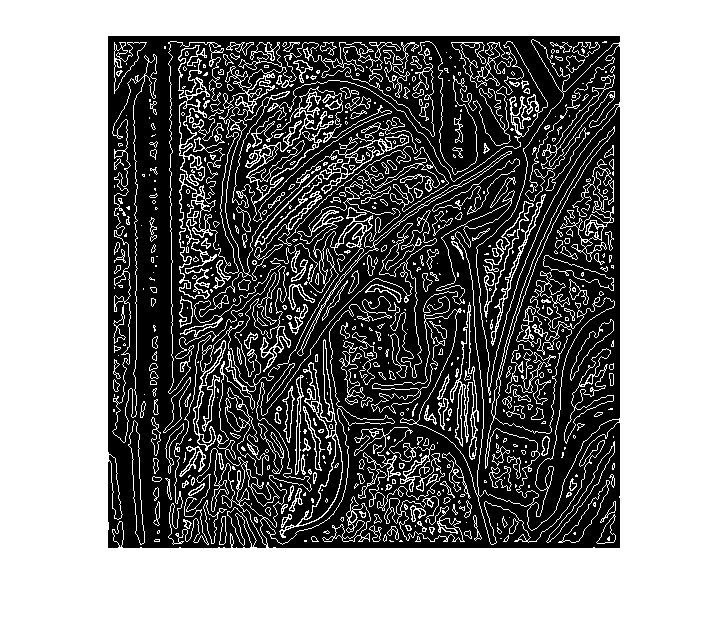
\includegraphics[width=\textwidth]{Images/lena_log_2.png}
            \subcaption{$\sigma=2$}
        \end{subfigure}
        \begin{subfigure}[b]{0.32\textwidth}
            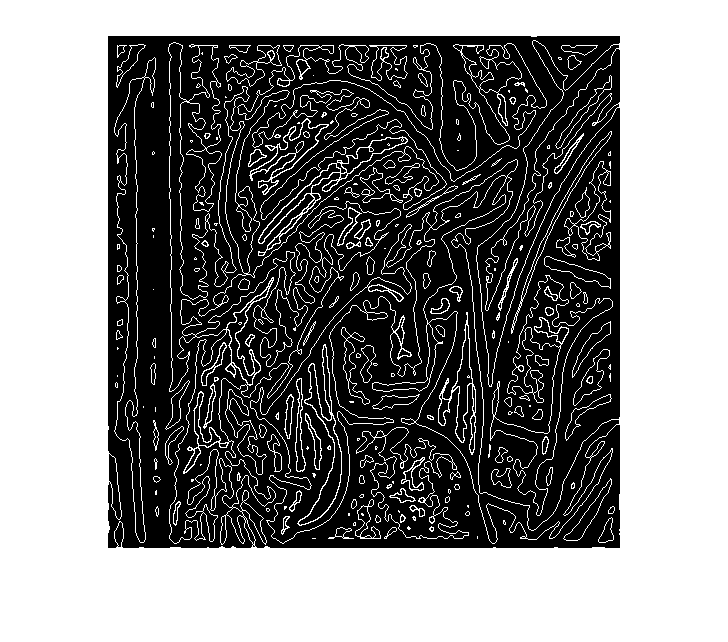
\includegraphics[width=\textwidth]{Images/lena_log_3.png}
            \subcaption{$\sigma=3$}
        \end{subfigure}
        \begin{subfigure}[b]{0.32\textwidth}
            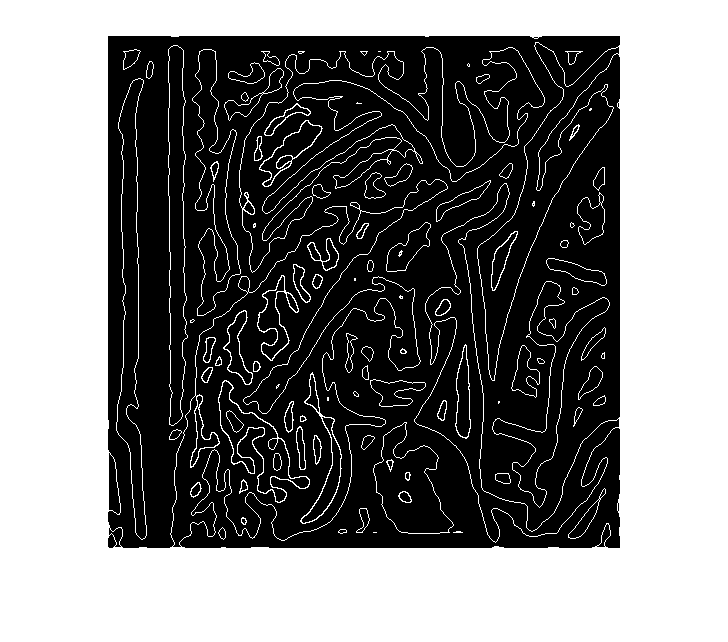
\includegraphics[width=\textwidth]{Images/lena_log_5.png}
            \subcaption{$\sigma=5$}
        \end{subfigure}
        \caption{Laplacian of Gaussian for edge detection using different values of $\sigma$.}
        \label{fig:log}
\end{figure}

\begin{figure}
        \centering
        \begin{subfigure}[b]{0.49\textwidth}
            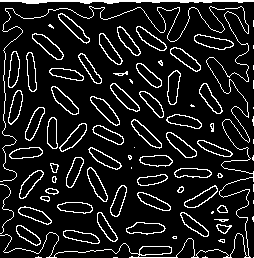
\includegraphics[width=\textwidth]{Images/rice_log.png}
            \subcaption{$\sigma=3$}
        \end{subfigure}
        \begin{subfigure}[b]{0.49\textwidth}
            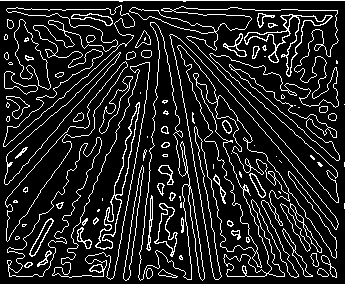
\includegraphics[width=\textwidth]{Images/road_log.png}
            \subcaption{$\sigma=3$}
        \end{subfigure}
        
        \caption{Laplacian of Gaussian for edge detection on \textsf{rice.png} and \textsf{road.png}.}
        \label{fig:log_r}
\end{figure}

\section{Frei-Chen Method}
In the Frei-Chen method, we create a 9D representation of the input image where the first two dimensions capture edge information while the others capture other structure information. For each pixel, an angle between the 9D vector and its projection to the two edge dimensions is computed as described in the assignment. These pixels are separated into edge vs. non-edge pixels through thresholding again. You can find the respective implementation in \textsf{frei\_chen(I, thresh)}, where \textsf{I} is the input image and \textsf{thresh} is the angle threshold in radiant. The different dimensions of the the 9D image representation are created by convolving \textsf{I} with the respective filter. Based on that, the angles are computed using the formula on the assignment sheet and edge pixels are extracted using \textsf{imbinarize(angles, thresh)}.

\paragraph{Discussion}
Finally, we can observe the results of the Frei-Chen method in Figure \ref{fig:freichen} and Figure \ref{fig:freichen_r}. It is able to capture dominant edges but lacks in detecting fine contour changes (cf. background). Again, if we have dominant intensity changes like in \textsf{rice.png}, the method works well.
\begin{figure}
    \centering
    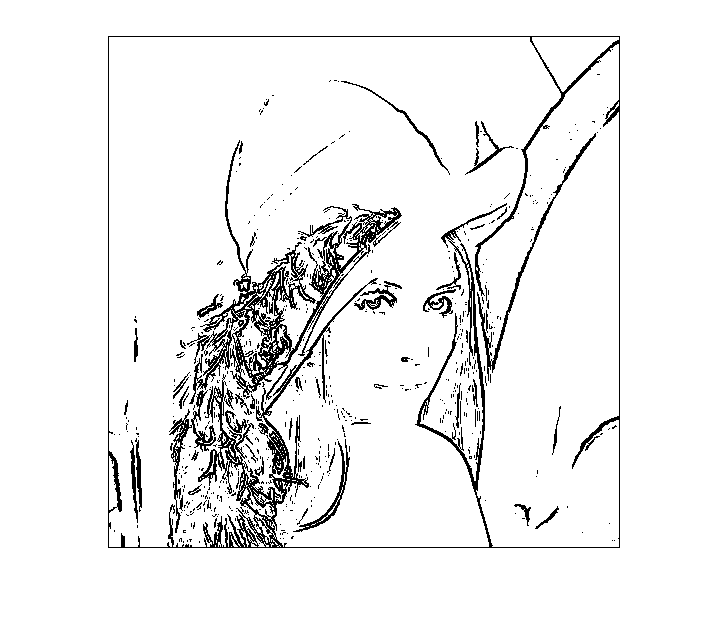
\includegraphics[width=0.5\textwidth]{Images/lena_frei_chen.png}
    \caption{Results of Frei-Chen method on \textsf{lena.png} with thresh=0.97.}
    \label{fig:freichen}
\end{figure}

\begin{figure}
        \centering
        \begin{subfigure}[b]{0.4\textwidth}
            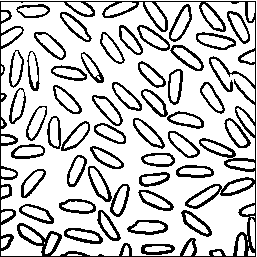
\includegraphics[width=\textwidth]{Images/rice_frei_chen.png}
            \subcaption{$t=0.98$}
        \end{subfigure}
        \begin{subfigure}[b]{0.4\textwidth}
            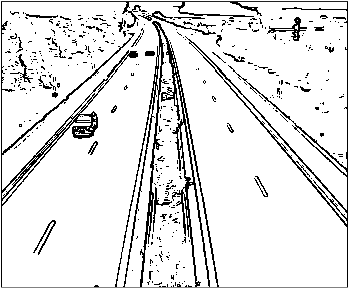
\includegraphics[width=\textwidth]{Images/road_frei_chen.png}
            \subcaption{$t=0.98$}
        \end{subfigure}
        \caption{Frei-Chen method on \textsf{rice.png} and \textsf{road.png}.}
        \label{fig:freichen_r}
\end{figure}

\section{Discussion}\label{sec:discussion}
In this section, the different edge detectors are compared in terms of speed and robustness to noise, computing the MSE between the edge image and the noised edge image. All methods are executed on the \textsf{lena.png} image with the above parameter settings. For the template methods (and also overall), Prewitt seems to be fastest. However, it does not produce the visually best results. The time complexity strongly increases for the Compass method, which was expected since we process $8$ filters. Frei-Chen method takes longest to compute. Looking at the robustness to noise, we can observe that the Frei-Chen method is surprisingly robust. In particular, for $\sigma = 25$ the edge image varies from the unnoised version the least. For the other methods, we can only detect small variations throughout the different $\sigma$-levels. However, Prewitt seems to be most sensitive to noise compared to all other images. \\
As for the last assignment, one should treat MSE with caution since it simply measures pixel difference quantitatively without taking into account positions. To conclude, one can say that all edge detectors we looked at are at some form parameter based. Thus, obtaining feasible results highly depends on how we choose the parameter depending on the respective image.

\begin{table}
\centering
\caption{Comparison of edge detection methods on lena-y.png}
\begin{tabular}{ c || c| c | c}
 Method & Parameters & Speed (ms) & MSE Noise with $\sigma=(5, 11, 25)$ \\ 
 \hline
 Template, Sobel & L1, $t=25$ & $8.49$ & ($0.58, 0.58, 0.58$) \\
 Template, Sobel & L2, $t=25$ & $11.31$ & ($0.49, 0.49, 0.48$)\\
 Template, Prewitt & L2, $t=25$ & $5.25$ & ($0.45, 0.46, 0.45$)\\
 Template, Roberts & L2, $t=25$ & $9.88$ & ($0.69, 0.69, 0.69$)\\
 Compass &  $t=25$ & $43.01$ & ($0.55, 0.53, 0.55$)\\
 LoG & $\sigma = 3$ & $30.62$ & ($0.18, 0.18, 0.17$) \\
 Frei-Chen & $t=0.97$ & $68.35$ & ($0.27, 0.25, 0.1$)\\
\end{tabular}
\label{tab:1}
\end{table}
\end{document}